\documentclass[border=6pt]{standalone}
\usepackage{fontspec}
\defaultfontfeatures{Ligatures=TeX}
\setmainfont{Palatino Linotype}
\usepackage{tikz}
\usetikzlibrary{arrows.meta, positioning, calc, shapes.geometric, fit,
                backgrounds, decorations.pathmorphing}
\definecolor{casink}{HTML}{1A1A22}
\definecolor{casaccent}{HTML}{6B3F8C}
\definecolor{casmuted}{HTML}{8A8A94}
\definecolor{caswash}{HTML}{F0ECF4}

\tikzset{
  casnode/.style={
    draw=casink, line width=0.5pt, rounded corners=1.2pt,
    fill=caswash, inner sep=3.2pt, font=\small, minimum height=6.5mm,
    align=center},
  casdomain/.style={
    casnode, minimum width=34mm, font=\small\bfseries},
  casflow/.style={
    -{Stealth[length=2.1mm,width=1.6mm]}, draw=casink, line width=0.55pt},
  casfeedback/.style={
    -{Stealth[length=2.1mm,width=1.6mm]}, draw=casmuted, line width=0.5pt,
    dashed, dash pattern=on 1.6pt off 1.4pt},
  casinvol/.style={
    {Stealth[length=1.8mm,width=1.4mm]}-{Stealth[length=1.8mm,width=1.4mm]},
    draw=casaccent, line width=0.5pt},
  caslabel/.style={font=\scriptsize, text=casmuted},
  cascap/.style={font=\scriptsize\itshape, text=casink},
}

% Every figure in this book uses the same wrapper so the list of figures and
% the numbering stay consistent.
\newcommand{\casfig}[3]{%
  \begin{figure}[htbp]
  \centering
  #2
  \caption{#3}\label{fig:#1}
  \end{figure}%
}

\begin{document}

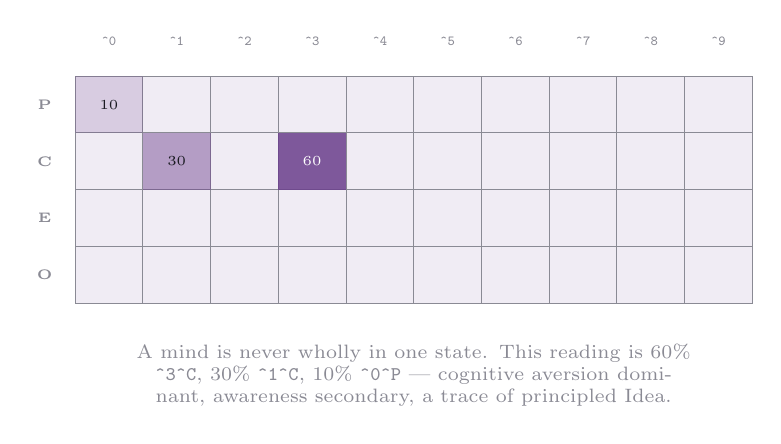
\begin{tikzpicture}[x=8.6mm, y=7.2mm]
  \foreach \c/\sym in {0/0,1/1,2/2,3/3,4/4,5/5,6/6,7/7,8/8,9/9} {
    \node[caslabel, font=\tiny] at (\c+0.5, 0.62) {\texttt{\^{}\sym}};
  }
  \foreach \r/\d in {0/P, 1/C, 2/E, 3/O} {
    \node[caslabel, font=\tiny\bfseries] at (-0.45, -\r-0.5) {\d};
    \foreach \c in {0,...,9} {
      \draw[draw=casmuted, line width=0.35pt, fill=caswash]
        (\c, -\r) rectangle (\c+1, -\r-1);
    }
  }
  % the worked example: 60% ^3^C, 30% ^1^C, 10% ^0^P
  \fill[casaccent, opacity=0.85] (3,-1) rectangle (4,-2);
  \node[font=\tiny, text=white] at (3.5,-1.5) {60};
  \fill[casaccent, opacity=0.45] (1,-1) rectangle (2,-2);
  \node[font=\tiny, text=casink] at (1.5,-1.5) {30};
  \fill[casaccent, opacity=0.18] (0,0) rectangle (1,-1);
  \node[font=\tiny, text=casink] at (0.5,-0.5) {10};
  \node[caslabel, anchor=north, text width=82mm, align=center]
    at (5, -4.55)
    {A mind is never wholly in one state. This reading is
     60\% \texttt{\^{}3\^{}C}, 30\% \texttt{\^{}1\^{}C}, 10\%
     \texttt{\^{}0\^{}P} --- cognitive aversion dominant, awareness
     secondary, a trace of principled Idea.};
\end{tikzpicture}

\end{document}
